\subsubsection{Varying message sizes}

In this experiment we show the effect of varying message sizes. The experiment is carried out in 512-node partition with 1 MPI/PAMI rank per node, 8 MB message size for all three patterns. The results for OPT and MPI are shown in Figure \ref{fig:messagesize}.
\begin{figure}[!htb]
\vspace{-0.15in}
\centering
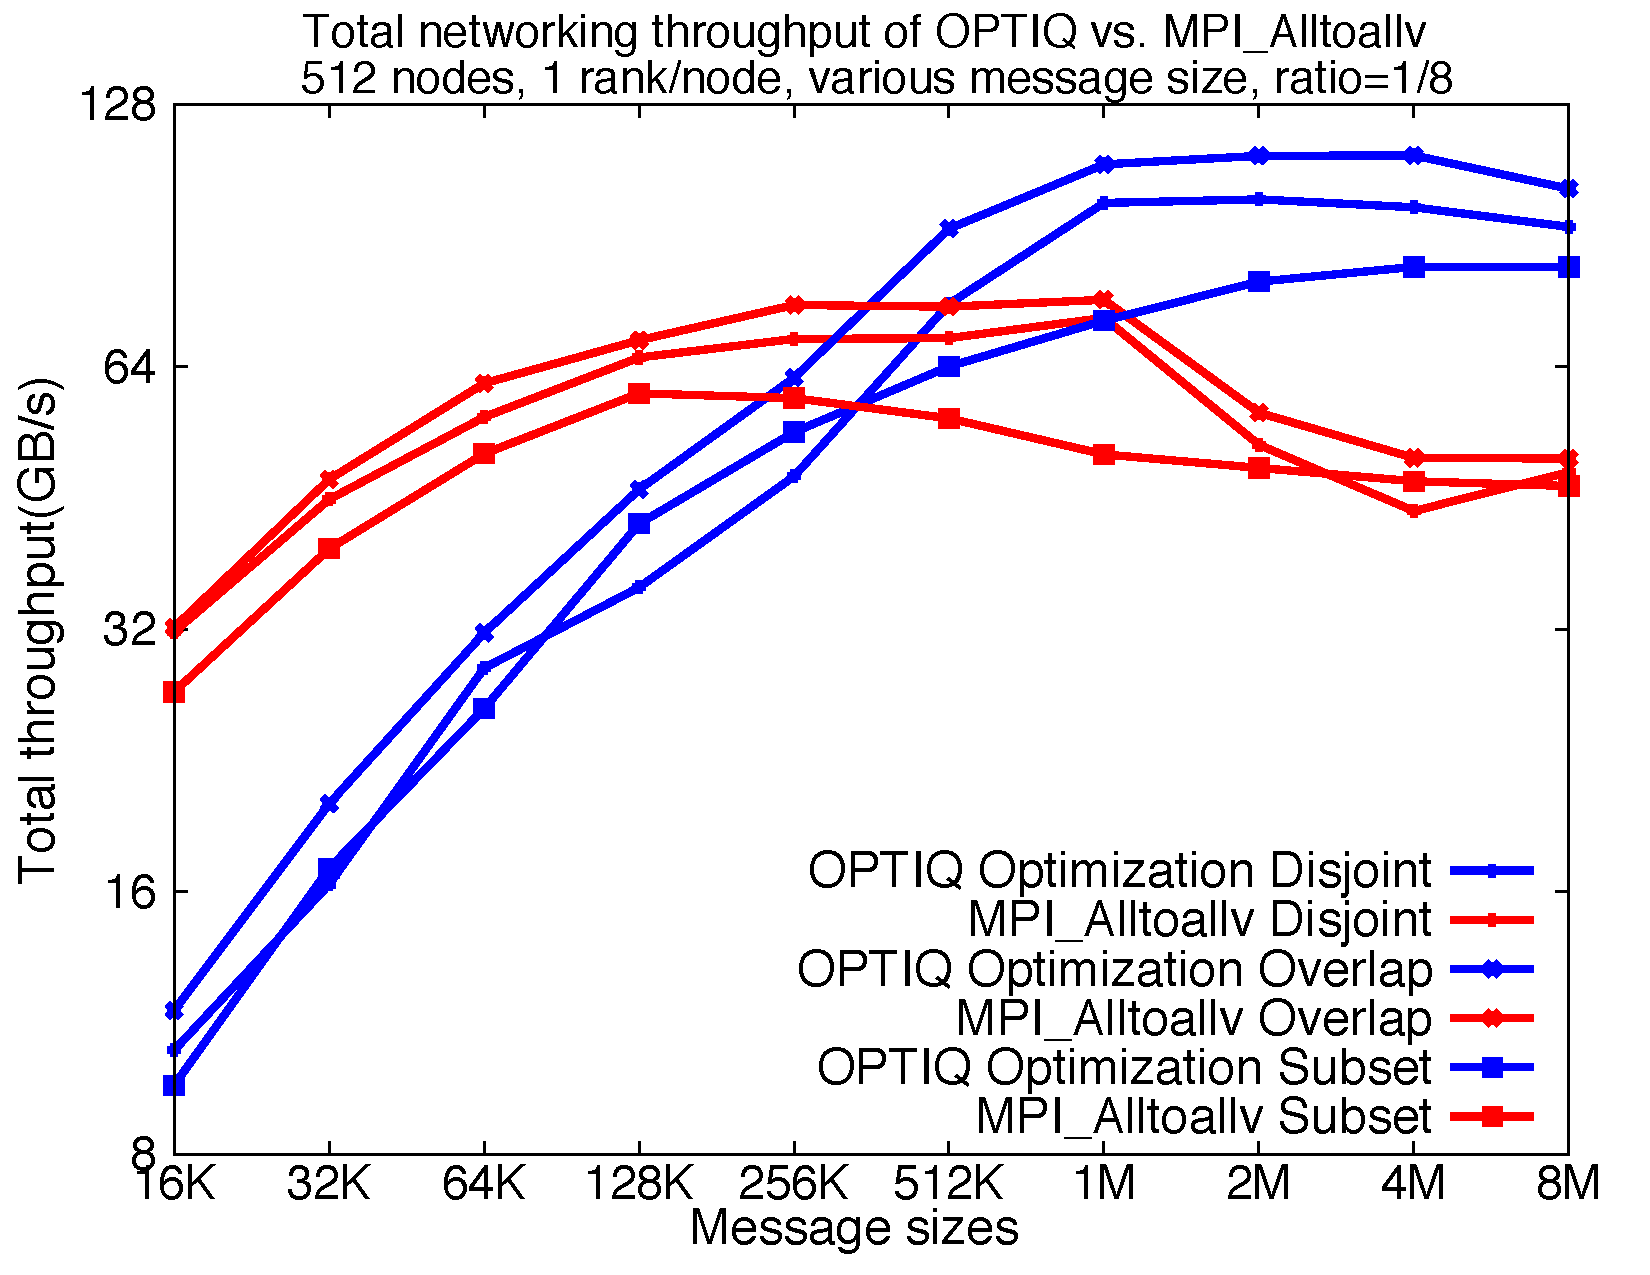
\includegraphics[scale=0.24]{figures/messagesize.pdf}
\vspace{-0.15in}
\caption{\small Total throughput with different message sizes from 16 KB -- 8 MB in disjoint, overlap and subset for OPT and MPI.}
\vspace{-0.15in}
\label{fig:messagesize}
\end{figure}
The throughput of transferring small messages in OPTIQ is lower than the default MPI\_Alltoallv due to overhead in data transfer by OPTIQ. MPI\_Alltoallv has better performance than OPTIQ when data size is less than 512 KB. 
%As shown in the figure, data transfer throughput flips in between 256 KB and 512 KB. 
%If the message size is less than 256 KB, MPI\_Alltoallv has better performance.
When the message size is greater than 512 KB, OPTIQ has better performance. The lower performance in OPT at smaller message sizes is due to overhead caused by additional messages, {\em send} and {\em forward} queueing, chunking of messages, and time to copy and inject messages at intermediate nodes.
